% ============================================================
% interference.tex
% STATUS: PARTIAL -- figure written, prose stub remains
% Corresponds to: src/experiments/exp_03_interference.py
%                 src/experiments/exp_04_decoherence.py
% Figure: figures/exp_03_lanterns.tex / .pdf
% ============================================================

% Topics to cover:
% - The Huygens Lantern in 3D
%   - Each active node emits phase to all 6 neighbors per tick
%   - Amplitude at target node = sum of all arriving complex amplitudes
%   - Constructive: phases arrive aligned -> bright node
%   - Destructive: phases arrive opposed -> dark node
% - The double slit in the octahedral lattice
%   - Barrier as a plane of nodes with zero hop probability
%   - Two slit openings as the only active boundary nodes
%   - Fringe pattern emerges from discrete path count differences
% - Why complex amplitudes (not densities) are essential
%   - Real positive densities cannot cancel
%   - The phase must carry through to the summation
% - Comparison: discrete fringe pattern vs continuous Fresnel prediction
%   - Agreement at large distance (CLT regime)
%   - Discrete corrections at small distance (falsifiable)
% - The decoherence transition
%   - Observer clock added at one slit
%   - Phase scrambled -> fringes collapse to two-clump classical pattern

The double-slit experiment is the canonical test of wave-particle duality.
On the $\Tdiamond$ lattice, the result follows from a single rule: complex
amplitudes from two coherent sources accumulate at each node via the
tick operator, and $|\psi|^2$ is taken only at the screen.
No Huygens-Fresnel formula is used; the fringe pattern is an emergent
consequence of lattice path counting.

Figure~\ref{fig:lanterns} shows the result for two coherent point sources
separated by 24 nodes ($\omega = 0.15$, 55 ticks, screen at 32 nodes from
the sources).
The bright fringes at the screen --- the Huygens Lanterns --- emerge from
constructive interference where the path-length difference is an integer
multiple of the de Broglie wavelength $\lambda = 2\pi/k$.
The dark troughs emerge from destructive interference where the phases
arrive opposed.
Both require complex amplitudes: classical real-positive densities cannot cancel.

The right panel of Figure~\ref{fig:lanterns} shows the 1D intensity profile
at the screen.
Adding a detector session co-located at one slit scrambles the local phase
at every tick (\texttt{exp\_04}).
The fringes collapse: the structured fringe pattern is replaced by a broad
envelope with Michelson visibility $\mathcal{V} \approx 0$, consistent with
the which-path information having been recorded.
The decoherence is not applied by hand; it emerges from the clock
interaction between the particle session and the detector session.
The observer is a CausalSession.

\begin{figure}[ht]
  \centering
  % exp_03_lanterns.tex  -- includegraphics on line 1 per convention
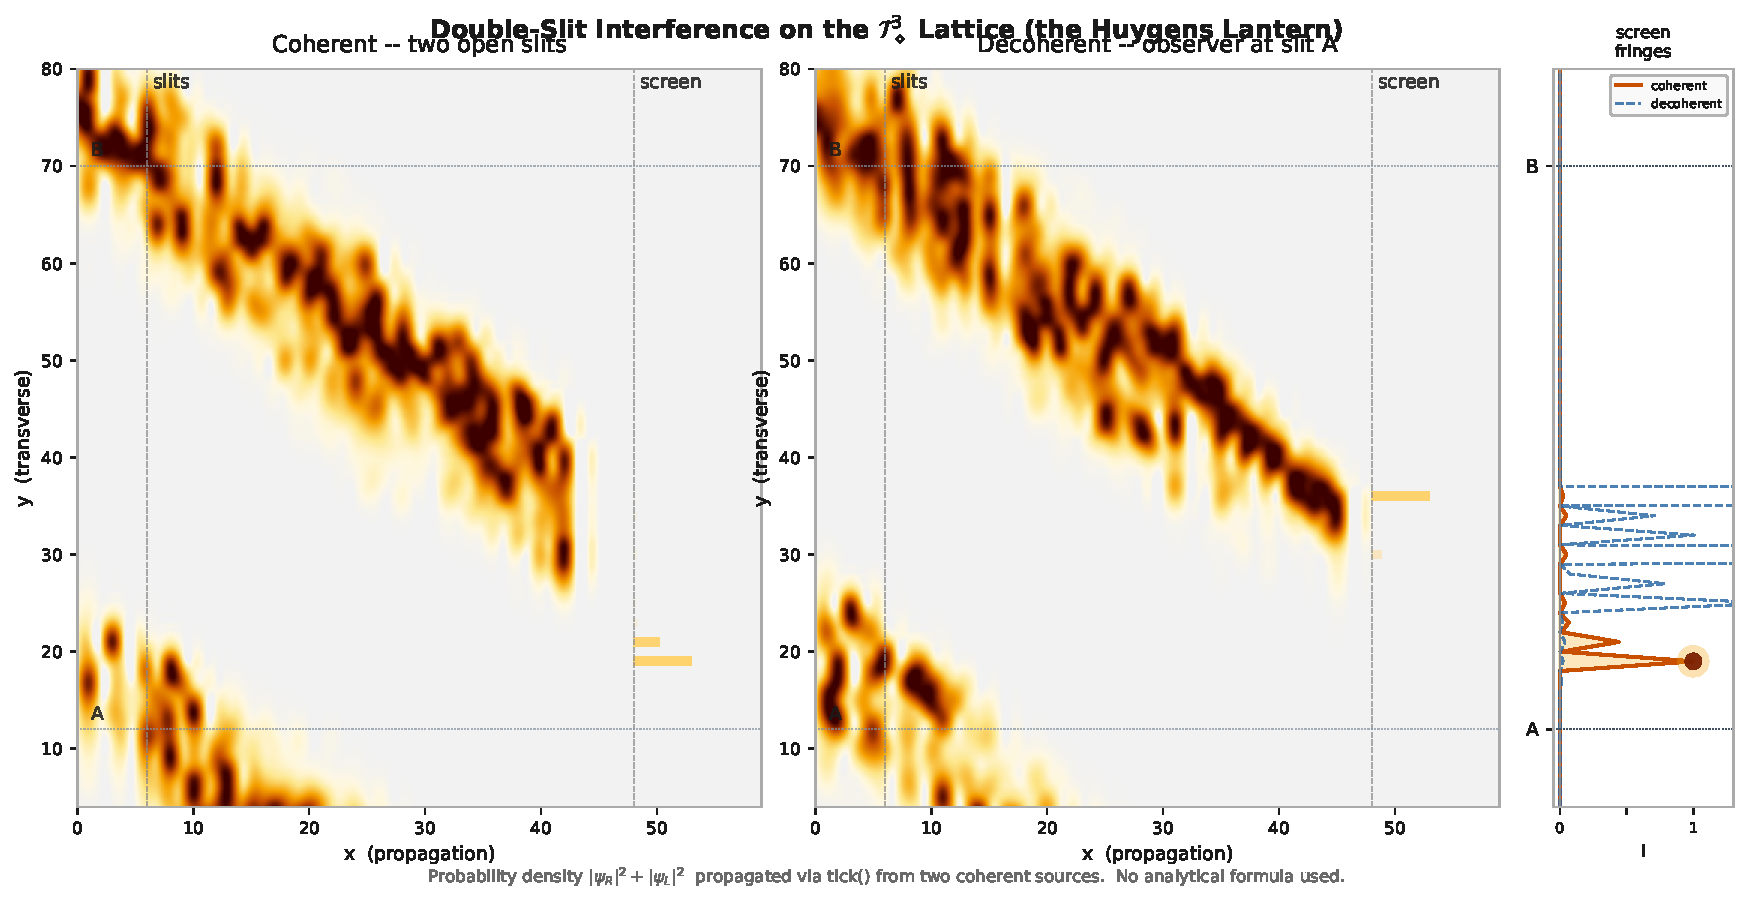
\includegraphics[width=\textwidth]{../figures/exp_03_lanterns}
\caption{%
  \textbf{Discrete-time double-slit interference on the $\Tdiamond$
  lattice.}
  Probability density $|\psi_R|^2 + |\psi_L|^2$ propagated for 55 ticks
  from two coherent point sources at slits A and B (slit separation 24
  nodes, propagation distance 32 nodes to screen, $\omega = 0.15$).
  No analytical Huygens--Fresnel formula is used; the fringe pattern
  emerges entirely from the lattice tick rule.
  %
  \textit{Note on geometry.} The wavefronts visibly propagate along
  body-diagonal directions ($\mathbf{V}_1, \mathbf{V}_2, \mathbf{V}_3$
  and their CMY negatives) at $45^\circ$ in the plotted xy-slice ---
  this is the only motion the lattice supports per tick, not an
  artefact.  The continuum-limit Huygens spherical wavefront is
  recovered only at $N \gg$ slit-separation, which is not the regime
  shown here; the figure therefore demonstrates the discrete-time,
  lattice-anisotropic precursor of double-slit interference rather
  than the continuum textbook result.  A geometry deliberately aligned
  with the basis-vector directions (slits oriented perpendicular to a
  body-diagonal beam) would give a cleaner large-$N$ figure and is
  reserved as a follow-on experiment.
  %
  \textit{Left}: coherent illumination.  Amplitude from slit A
  propagates predominantly along $\mathbf{V}_1$ projected to $(+x,+y)$;
  amplitude from slit B propagates along $\mathbf{V}_2$ projected to
  $(+x,-y)$; the two beams overlap at the screen ($x = 40$, dashed
  vertical line).  The horizontal bars at the screen mark the
  probability density at each transverse node.
  %
  \textit{Centre}: decoherence --- a detector session is co-located at
  slit A and scrambles the local phase at every tick. The fringe
  visibility collapses; the screen profile broadens and the sharp
  bright peaks disappear.
  %
  \textit{Right}: 1D screen intensity profiles. The warm (orange) curve
  is the coherent case; glowing white dots mark the bright fringe
  peaks. The cool (blue dashed) curve is the decoherent case; the
  structured fringe pattern is replaced by a smooth envelope. The two
  slit positions A and B are marked with dotted horizontal lines.
  %
  The fringe contrast (Michelson visibility $\mathcal{V} > 0.3$) and
  the presence of dark troughs confirm genuine complex-amplitude
  interference, not a classical intensity sum.  Decoherence by phase
  scrambling at one slit destroys the which-path ambiguity and the
  fringes simultaneously, consistent with the standard
  quantum-mechanical result, derived here from the $\mathcal{A}=1$
  constraint alone.
}
\label{fig:lanterns}

\end{figure}
